\section{A little bit of math}

\begin{frame}{Composition of functions} 
	\begin{columns}
		\begin{column}{.5\textwidth}
			Consider the following  functions 
			\begin{align*}
				f(x)=& log(x) \\
				g(x)=&  x^2 \\
				g(f(x)) =& (log(x))^2 \\  
			\end{align*}
		\end{column}
		\begin{column}{.5\textwidth}
			\begin{figure}
				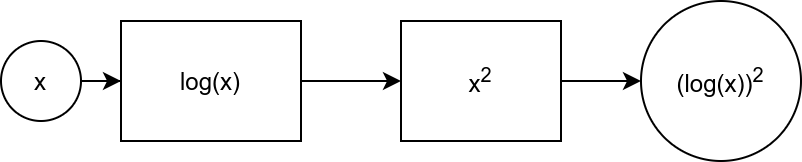
\includegraphics[width=.8\textwidth, center]{figures/function_composition}
				\caption*{Composition blocks}
			\end{figure}
		\end{column}
	\end{columns}

\end{frame}